%%%%%%%%%%%%%%%%%%%%%%%%%%%%%%%%%%%%%%%%%%%%%%%%%%%%%%%%%%%%
% Preamble:
%%%%%%%%%%%%%%%%%%%%%%%%%%%%%%%%%%%%%%%%%%%%%%%%%%%%%%%%%%%%

% KOMA article class
% see also:
% http://mirror.ctan.org/macros/latex/contrib/koma-script/scrguide.pdf
\documentclass{scrartcl}

\usepackage[utf8]{inputenc}
\usepackage[T1]{fontenc}

% latin modern - 'The fonts, as compared to the CM family,
% contain a lot of additional characters, mainly accented
% ones.' http://www.ctan.org/tex-archive/fonts/lm/
\usepackage{lmodern}

\usepackage[english]{babel}
%\usepackage[ngerman]{babel}

% e.g.: \includegraphics ...
\usepackage{graphicx}

% e.g. \align ...
\usepackage{amsmath}

% verbatim program code:
% \usepackage{listings}
% nicer tables:
% \usepackage{colortbl}
\usepackage{booktabs}

\usepackage{biblatex}
\bibliography{biblio}

% always last:
% e.g. \url, \href, inter-PDF-links ...
\usepackage{hyperref}

%%%%%%%%%%%%%%%%%%%%%%%%%%%%%%%%%%%%%%%%%%%%%%%%%%%%%%%%%%%%
% Document:
%%%%%%%%%%%%%%%%%%%%%%%%%%%%%%%%%%%%%%%%%%%%%%%%%%%%%%%%%%%%

\subject{Ausarbeitung}
\titlehead{Seminar Parallele Algorithmen SS 2012}
\title{OpenCL}
\subtitle{An Overview}
\author{Joe User}
%\date{}
%\publishers{}

\begin{document}

\maketitle

\begin{abstract}
Lorem ipsum dolor sit amet, consectetur adipisicing elit, sed do eiusmod tempor incididunt ut labore et dolore magna aliqua. Ut enim ad minim veniam, quis nostrud exercitation ullamco laboris nisi ut aliquip ex ea commodo consequat.
\end{abstract}

\section{Introduction}

\begin{figure}
  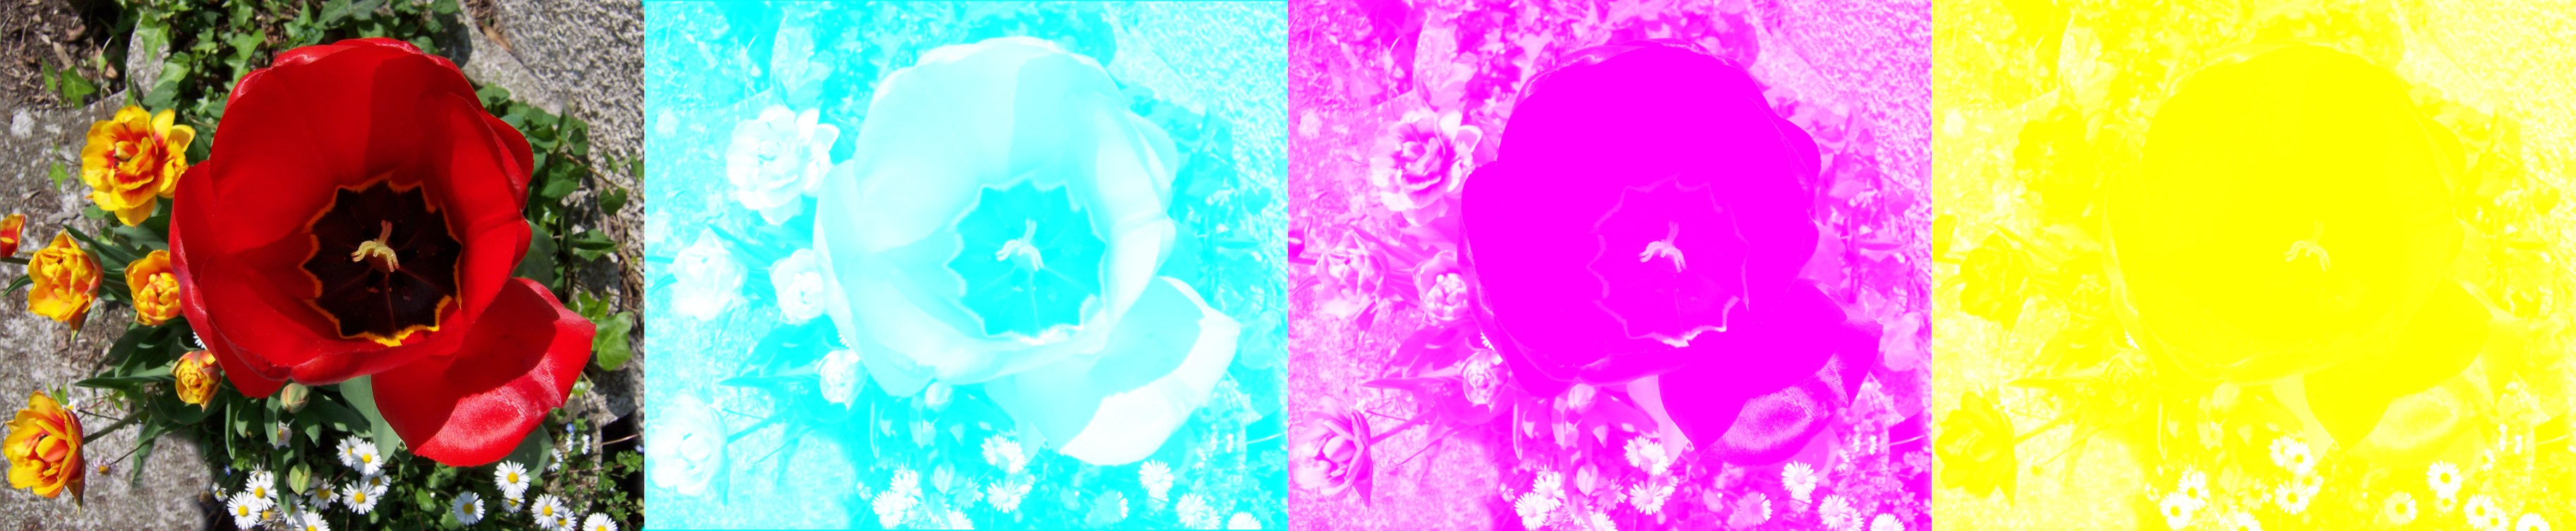
\includegraphics[width=1\textwidth]{SubtractiveColorSynthesis_CMYpositives.jpg}
  \caption{Random figure caption text {\tiny (Image is licensed under CC
  SA-BY 3.0 and is available from
  \url{http://commons.wikimedia.org/wiki/File:SubtractiveColorSynthesis_CMYpositives.jpg})}}
  \label{fig:foo}
\end{figure}

Duis aute irure dolor in reprehenderit in voluptate velit esse
cillum dolore eu fugiat nulla pariatur (see Figure
\ref{fig:foo}). Excepteur sint occaecat
cupidatat non proident, sunt in culpa qui officia deserunt mollit
anim id est laborum\cite{NUS:PIE:GRI:KLE:1978}.

Lorem ipsum dolor sit amet, consectetur adipisicing elit, sed do
eiusmod tempor incididunt ut labore et dolore magna aliqua. Ut
enim ad minim veniam, quis nostrud exercitation ullamco laboris
nisi ut aliquip ex ea commodo consequat\cite{YOU:1967}.

\subsection{Related Work}

Lorem ipsum dolor sit amet, consectetur adipisicing elit, sed do
eiusmod tempor incididunt ut labore et dolore magna aliqua. Ut
enim ad minim veniam, quis nostrud exercitation ullamco laboris
nisi ut aliquip ex ea commodo consequat. Duis aute irure dolor in
reprehenderit in voluptate velit esse cillum dolore eu fugiat
nulla pariatur. Excepteur sint occaecat cupidatat non proident,
sunt in culpa qui officia deserunt mollit anim id est laborum.

\begin{table}
  % Note: tables have their caption above (and figures below)
  \caption{Language keyword table}
  \label{tab:lang}
  \begin{tabular}{lr}
    \toprule
    Sprache  & \#Keywords \\
    \midrule
    Haskell  & 21         \\
    Scheme   & 23         \\
    C (C89)  & 32         \\
    Java     & 50         \\
    Ada      & 72         \\
    C++      & 74         \\
    \bottomrule
  \end{tabular}
\end{table}

\section{OpenCL}

\begin{align}
  \text{es}(n) & = \frac{1}{(1-p) + \frac{p}{n}} \\ & \le \frac{1}{1-p} \\
  \text{es}^{*}(n) & = \frac{1}{(1-p) + \frac{p}{n} + \phi(n)}
\end{align}

\section{Conclusion}

\printbibliography

\end{document}


